\documentclass[10pt]{article}
\usepackage[letterpaper,margin=0.85in]{geometry}
\usepackage{times}
\usepackage{graphicx}
\usepackage{booktabs}
\usepackage{amsmath}
\usepackage{amssymb}
\usepackage{caption}
\usepackage{subcaption}
\usepackage{float}
\usepackage{enumitem}
\usepackage{hyperref}
\usepackage{xcolor}
\usepackage{tikz}
\usetikzlibrary{positioning,arrows.meta,fit,calc}
\hypersetup{colorlinks=true,linkcolor=black,citecolor=black,urlcolor=black}
\captionsetup{font=footnotesize,labelfont=bf}
\setlength{\parindent}{1em}
\setlength{\parskip}{0pt}
\setlength{\textfloatsep}{7pt}
\setlength{\floatsep}{6pt}
\setlength{\intextsep}{6pt}
\setlength{\emergencystretch}{2em}
\setlist[itemize]{leftmargin=1.1em,itemsep=1pt,topsep=2pt}
\setlist[enumerate]{leftmargin=1.2em,itemsep=1pt,topsep=2pt}
\renewcommand{\thesection}{\Roman{section}}
\renewcommand{\thesubsection}{\Alph{subsection}}

\graphicspath{%
  {outputs/figures/training/deit_pretrained/}%
  {outputs/figures/xai/}%
  {outputs/figures/evaluation/axis1_stability/}%
  {outputs/figures/evaluation/axis2_faithfulness/}%
  {outputs/figures/evaluation/axis4_representation/}%
  {outputs/explanations/pretrained_best/token_transformation/}%
  {outputs/explanations/pretrained_best/attention_rollout/}%
  {outputs/explanations/pretrained_best/attention_weights/}%
  {outputs/explanations/pretrained_best/tam/}%
  {outputs/explanations/pretrained_best/occlusion/}%
  {outputs/explanations/pretrained_best/causal_patch_impact/}%
  {outputs/explanations/pretrained_best/patch_attribution/}%
  {outputs/explanations/pretrained_best/shap/}%
  {outputs/explanations/pretrained_best/context_swap/}%
  {outputs/explanations/pretrained_best/counterfactual/}%
}

\newcommand{\methodfig}[4]{%
\textbf{#1} &
\includegraphics[width=.265\linewidth]{#2} &
\includegraphics[width=.265\linewidth]{#3} &
\includegraphics[width=.265\linewidth]{#4}\\[-2pt]}

\newcommand{\sampletriplet}[3]{%
\begin{minipage}[t]{.32\linewidth}\centering\includegraphics[width=\linewidth]{#1}\\[-1pt]\footnotesize (a) Cactus / dim\end{minipage}\hfill
\begin{minipage}[t]{.32\linewidth}\centering\includegraphics[width=\linewidth]{#2}\\[-1pt]\footnotesize (b) Airplane / autumn\end{minipage}\hfill
\begin{minipage}[t]{.32\linewidth}\centering\includegraphics[width=\linewidth]{#3}\\[-1pt]\footnotesize (c) Crab / dim\end{minipage}}

\newcommand{\samplesix}[6]{%
\begin{minipage}[t]{.31\linewidth}\centering\includegraphics[width=\linewidth]{#1}\\[-1pt]\footnotesize (a) Cactus / dim\end{minipage}\hfill
\begin{minipage}[t]{.31\linewidth}\centering\includegraphics[width=\linewidth]{#2}\\[-1pt]\footnotesize (b) Airplane / autumn\end{minipage}\hfill
\begin{minipage}[t]{.31\linewidth}\centering\includegraphics[width=\linewidth]{#3}\\[-1pt]\footnotesize (c) Crab / dim\end{minipage}\\[5pt]
\begin{minipage}[t]{.31\linewidth}\centering\includegraphics[width=\linewidth]{#4}\\[-1pt]\footnotesize (d) Horse / water\end{minipage}\hfill
\begin{minipage}[t]{.31\linewidth}\centering\includegraphics[width=\linewidth]{#5}\\[-1pt]\footnotesize (e) Fishing rod / water\end{minipage}\hfill
\begin{minipage}[t]{.31\linewidth}\centering\includegraphics[width=\linewidth]{#6}\\[-1pt]\footnotesize (f) Train / autumn\end{minipage}}

\newcommand{\inplacesix}[8]{%
\begin{center}
\samplesix{#1}{#2}{#3}{#4}{#5}{#6}
\captionof{figure}{#7}
\label{#8}
\end{center}}

\newcommand{\inplacetriplet}[5]{%
\begin{center}
\sampletriplet{#1}{#2}{#3}
\captionof{figure}{#4}
\label{#5}
\end{center}}

\newcommand{\contextrow}[5]{%
\begin{minipage}[t]{.19\linewidth}\centering\includegraphics[width=\linewidth]{#1}\\[-1pt]\footnotesize (a) Dim\end{minipage}\hfill
\begin{minipage}[t]{.19\linewidth}\centering\includegraphics[width=\linewidth]{#2}\\[-1pt]\footnotesize (b) Grass\end{minipage}\hfill
\begin{minipage}[t]{.19\linewidth}\centering\includegraphics[width=\linewidth]{#3}\\[-1pt]\footnotesize (c) Rock\end{minipage}\hfill
\begin{minipage}[t]{.19\linewidth}\centering\includegraphics[width=\linewidth]{#4}\\[-1pt]\footnotesize (d) Water\end{minipage}\hfill
\begin{minipage}[t]{.19\linewidth}\centering\includegraphics[width=\linewidth]{#5}\\[-1pt]\footnotesize (e) Outdoor\end{minipage}}

\title{\vspace{-0.25in}\bfseries When Context Becomes Evidence: Patch-Level XAI for DeiT on NICO++}
\author{Prerak Patel\\
Florida Institute of Technology\\
\texttt{ppatel2025@my.fit.edu}}
\date{}

\begin{document}
\maketitle

\begin{abstract}
Vision Transformers (ViTs) classify images through patch tokens, which positions them well for patch-level explainability while leaving them exposed to context shortcuts. This paper studies an ImageNet-pretrained DeiT-Small/16 fine-tuned on NICO++, a 60-class object dataset with six annotated contexts. The model reaches 90.47\% test accuracy and 0.9064 macro-F1, though performance varies by context: the worst context is \emph{dim} at 88.92\%, and group accuracy spans 0.75 to 1.00. Eight patch-level explanation methods are compared token transformation, raw CLS attention, attention rollout, Transition Attention Maps (TAM), occlusion sensitivity, causal patch impact, gradient $\times$ input, and kernel SHAP using top-$k$ deletion AUC on 200 stratified samples. TAM is the most faithful method (AUC 0.1579), followed by attention rollout (0.2022); SHAP is weakest at 0.2562 under a 512-coalition budget. Patch-level context swapping shows that 20\% of same-class cross-context swaps flip the prediction, with the largest probability drops in the \emph{water} context. High accuracy does not guarantee context-invariant reasoning, and gradient-weighted transformer attention proves the most reliable explanation family for this DeiT/NICO++ setting.
\end{abstract}

\noindent\textbf{Index Terms--} Vision Transformer, DeiT, NICO++, explainable AI, attention rollout, TAM, occlusion, SHAP, context shift.

\section{Introduction}
Modern image classifiers often learn shortcuts: they exploit background, co-occurrence, illumination, or dataset collection artifacts when those cues reduce training loss \cite{geirhos2020shortcut}. NICO++ is designed to expose this failure mode by pairing each object category with context labels such as \emph{grass}, \emph{water}, \emph{rock}, \emph{dim}, \emph{outdoor}, and \emph{autumn} \cite{zhang2023nico}. A classifier can therefore be accurate overall while still relying on context in specific class-context cells.

The central question is specific: when a DeiT-Small/16 model predicts a NICO++ class, which patches provide the evidence? ViTs are well suited for this because the image is already a $14\times14$ patch grid. But ViT explanations are not interchangeable. Raw attention is easy to visualize but not necessarily causal. Perturbation methods have clearer causal semantics but are slower and sensitive to the replacement baseline. SHAP has game-theoretic guarantees but is hard to estimate over 196 dependent patches. We compare all three families through qualitative sample panels and a deletion-AUC faithfulness protocol.

The main contributions are:
\begin{enumerate}
    \item an IEEE-style, reproducible report of DeiT-Small/16 fine-tuning on NICO++ with class-context metrics;
    \item a unified comparison of patch-level ViT explanations, including three representative sample panels per method;
    \item a detailed analysis showing that TAM is the strongest explanation method by deletion AUC and that water-context patches induce the largest prediction shifts under patch-level swapping.
\end{enumerate}

\section{Literature Review and Positioning}
\label{sec:lit}
This project builds on work in Vision Transformers, transformer explanation, model-agnostic attribution, and shortcut learning. The review below makes explicit what is adopted from prior work and how this report differs.

\textbf{Vision Transformer and DeiT.} Dosovitskiy et al. introduced the Vision Transformer, splitting images into fixed-size patches processed as tokens through a standard transformer encoder \cite{dosovitskiy2021image}. Touvron et al. showed that ViTs can be trained on standard ImageNet data without the large-scale compute of the original ViT, using DeiT with knowledge distillation through attention \cite{touvron2021training}. This report uses DeiT-Small/16 with ImageNet initialization. The patch-token structure carries through to every explanation: all saliency maps are on the $14\times14$ patch grid. The focus is not on architecture or top-1 accuracy but on whether a fine-tuned ViT leans on object patches or context patches when making decisions.

\textbf{Attention flow and attention rollout.} Abnar and Zuidema proposed attention rollout as a way to trace information flow through stacked transformer layers, accounting for residual connections and multi-head averaging \cite{abnar2020quantifying}. This report uses rollout as the main parameter-free attention baseline. The key difference from the original paper is that rollout is evaluated here against gradient-weighted, perturbation, and SHAP explanations through a deletion-AUC protocol a comparison Abnar and Zuidema did not attempt. Rollout performs well but not best: stable and visually reasonable, but it loses to TAM because it does not filter attention by target-class gradient sign.

\textbf{Transformer interpretability beyond raw attention.} Chefer et al. showed that raw attention is not sufficient for faithful ViT explanations and proposed relevance propagation through transformer components \cite{chefer2021transformer}. The central warning from that work that attention maps should not be taken as causal evidence shapes the design of this study. Rather than implementing full relevance propagation, this report tests several explanation families side by side under one deletion protocol, with context swaps as an additional intervention check. The tradeoff is reproducibility: fewer moving parts make the method comparison cleaner.

\textbf{Transition Attention Maps.} Yuan et al. proposed Transition Attention Maps (TAM), which weight attention by positive target-class gradients to isolate the attention paths that actually support the prediction \cite{yuan2021tam}. This report applies TAM to the NICO++ context-shift problem and benchmarks it against six other methods under a deletion-AUC protocol. TAM produces cleaner maps in the qualitative figures and achieves the lowest deletion AUC, making it the recommended method for this DeiT/NICO++ setting.

\textbf{Causal ViT explanations.} Xie et al. framed ViT explanation as a causal patch intervention problem in ViT-CX, arguing that a patch matters only if intervening on it changes the prediction \cite{xie2023vitcx}. This report follows that framing, but the pipeline falls back to input-space patch replacement when latent intervention hooks are not available. As a result, causal patch impact behaves nearly identically to occlusion both methods score deletion AUC 0.2264. The comparison remains useful: it shows that causal patch impact adds something only when true latent-token intervention is implemented.

\textbf{Model-agnostic attribution.} Lundberg and Lee introduced SHAP as a Shapley-value framework for feature attribution \cite{lundberg2017unified}. This report applies it at the patch level, treating each of the 196 ViT patches as one feature. Spatial correlation among patches and the small coalition budget (512 samples for a 196-dimensional space) make the estimate noisy, and the results show it: SHAP has the weakest deletion AUC and the noisiest visual maps.

\textbf{Shortcut learning and NICO++.} Geirhos et al. characterized shortcut learning the tendency of deep networks to exploit non-causal cues that happen to correlate with labels and showed it is pervasive in standard training \cite{geirhos2020shortcut}. Zhang et al. designed NICO++ specifically to expose this: by pairing object classes with annotated contexts, the benchmark lets researchers test whether models generalize across scenes or rely on background patterns \cite{zhang2023nico}. This report uses NICO++ for a patch-level audit rather than a domain-generalization leaderboard. The same-object cross-context panels in Section~\ref{sec:same-object} extend the standard evaluation by showing how explanations shift when the object label is fixed but the background changes.

\section{Dataset and Training}
The NICO++ data are reorganized into \texttt{<context>/<class>/<image>} form, deduplicated by file hash, and split with class $\times$ context stratification. The resulting splits contain 57,762 train images, 13,330 validation images, and 17,774 test images. Training uses resize to 256, random crop to $224\times224$, RandAugment ($n=2$, $m=9$), horizontal flip, ImageNet normalization, and random erasing ($p=0.25$). Validation, testing, and XAI use deterministic resize, center crop, and normalization. Mixup and CutMix are deliberately excluded because they break the one-image, one-label, one-patch-grid assumption needed for patch-level explanations.

The model is \texttt{deit\_small\_patch16\_224} initialized with ImageNet-1k \texttt{fb\_in1k} weights from \texttt{timm}. The 1000-way ImageNet head is replaced by a 60-way linear head. Training uses AdamW with learning rate $3\times10^{-5}$ for the backbone, $10^{-4}$ for the head, weight decay 0.05, cosine decay, two warm-up epochs, batch size 64, and 30 epochs. Checkpoints are saved by validation accuracy, macro-F1, loss, and worst-context accuracy. XAI results are generated from the best validation macro-F1 checkpoint.

\subsection{Implementation Details}
The implementation is organized as a reproducible PyTorch pipeline. Dataset preparation scripts deduplicate files, create class-context stratified CSV splits, and load images with deterministic transforms for evaluation. Training scripts save per-epoch metrics and multiple checkpoints, including best validation accuracy, macro-F1, loss, and worst-context accuracy. XAI scripts load the selected checkpoint, run each attribution method on 200 stratified samples, save per-sample heatmaps and overlays, and compute evaluation summaries.

All explanation maps are normalized to a common $14\times14$ patch grid before comparison. Faithfulness is computed by masking the top-ranked patches at fixed fractions and measuring the target-class probability drop. Stability is computed under Gaussian input perturbations for fast methods. Context-swap experiments pair same-class images from different contexts and replace the top-attributed patches to measure whether highlighted regions transfer object evidence or context evidence. This design ensures every method is evaluated on the same model, samples, patch grid, and deletion protocol.

\begin{figure}[H]
\centering
\resizebox{.96\textwidth}{!}{%
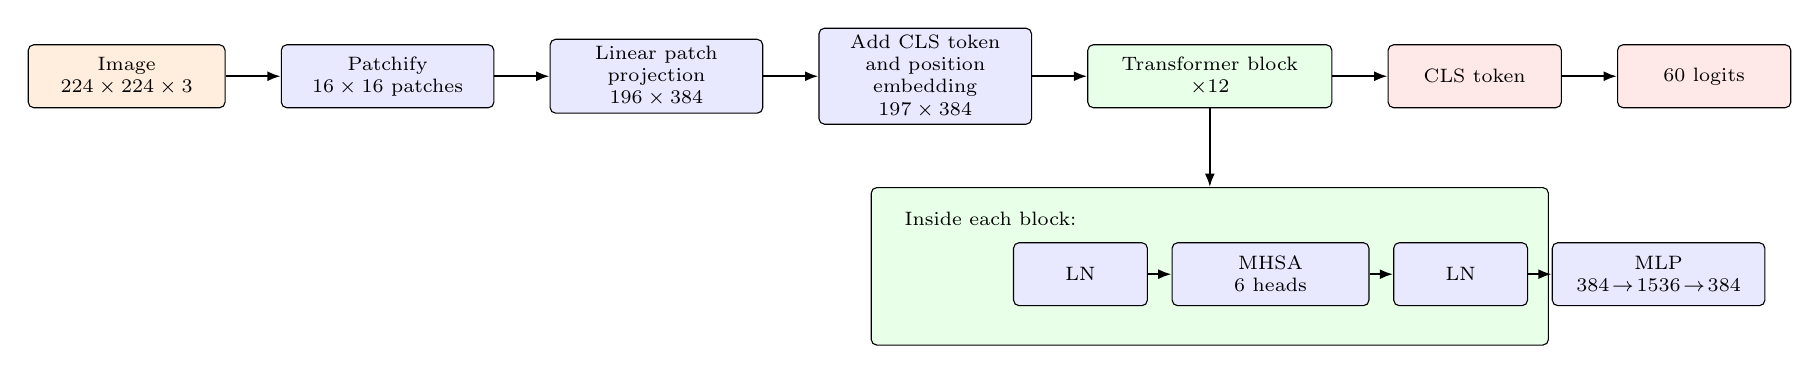
\begin{tikzpicture}[
  font=\scriptsize,
  node distance=5mm and 7mm,
  box/.style={draw, rounded corners=2pt, align=center, minimum height=8mm, inner sep=2.5pt},
  data/.style={box, fill=orange!13, minimum width=25mm},
  proc/.style={box, fill=blue!9, minimum width=27mm},
  block/.style={box, fill=green!9, minimum width=31mm},
  head/.style={box, fill=red!9, minimum width=22mm},
  arr/.style={-{Latex[length=1.7mm]}, thick}]
\node[data] (img) {Image\\$224\times224\times3$};
\node[proc, right=of img] (patch) {Patchify\\$16\times16$ patches};
\node[proc, right=of patch] (embed) {Linear patch\\projection\\$196\times384$};
\node[proc, right=of embed] (pos) {Add CLS token\\and position\\embedding\\$197\times384$};
\node[block, right=of pos] (b1) {Transformer block\\$\times 12$};
\node[head, right=of b1] (cls) {CLS token};
\node[head, right=of cls] (logits) {60 logits};
\draw[arr] (img) -- (patch);
\draw[arr] (patch) -- (embed);
\draw[arr] (embed) -- (pos);
\draw[arr] (pos) -- (b1);
\draw[arr] (b1) -- (cls);
\draw[arr] (cls) -- (logits);

\node[block, below=10mm of b1, minimum width=86mm, minimum height=20mm] (detail) {};
\node[anchor=west] at ([xshift=-40mm,yshift=6mm]detail.center) {Inside each block:};
\node[proc, anchor=west, minimum width=17mm] (ln1) at ([xshift=-25mm,yshift=-1mm]detail.center) {LN};
\node[proc, right=3mm of ln1, minimum width=25mm] (msa) {MHSA\\6 heads};
\node[proc, right=3mm of msa, minimum width=17mm] (ln2) {LN};
\node[proc, right=3mm of ln2, minimum width=27mm] (mlp) {MLP\\$384\!\to\!1536\!\to\!384$};
\draw[arr] (ln1) -- (msa);
\draw[arr] (msa) -- (ln2);
\draw[arr] (ln2) -- (mlp);
\draw[arr] (b1.south) -- (detail.north);
\end{tikzpicture}
}
\caption{DeiT-Small/16 architecture used in this study. The image becomes 196 patch tokens plus one CLS token. The 12 transformer blocks each contain LayerNorm, 6-head self-attention, residual connections, and a 4$\times$ MLP. Explanations are reported on the $14\times14$ patch grid.}
\label{fig:architecture}
\end{figure}

\section{Explainability Methods}
\label{sec:methods}
Let an image $\mathbf{x}$ be split into $P=196$ patches. The class logit for target class $y$ is $f_y(\mathbf{x})$ and the probability is $p_y(\mathbf{x})$. Every method produces a saliency map $s\in\mathbb{R}^{14\times14}$, which is min-max normalized before visualization and deletion scoring.

\begin{figure}[H]
\centering
\resizebox{.98\textwidth}{!}{%
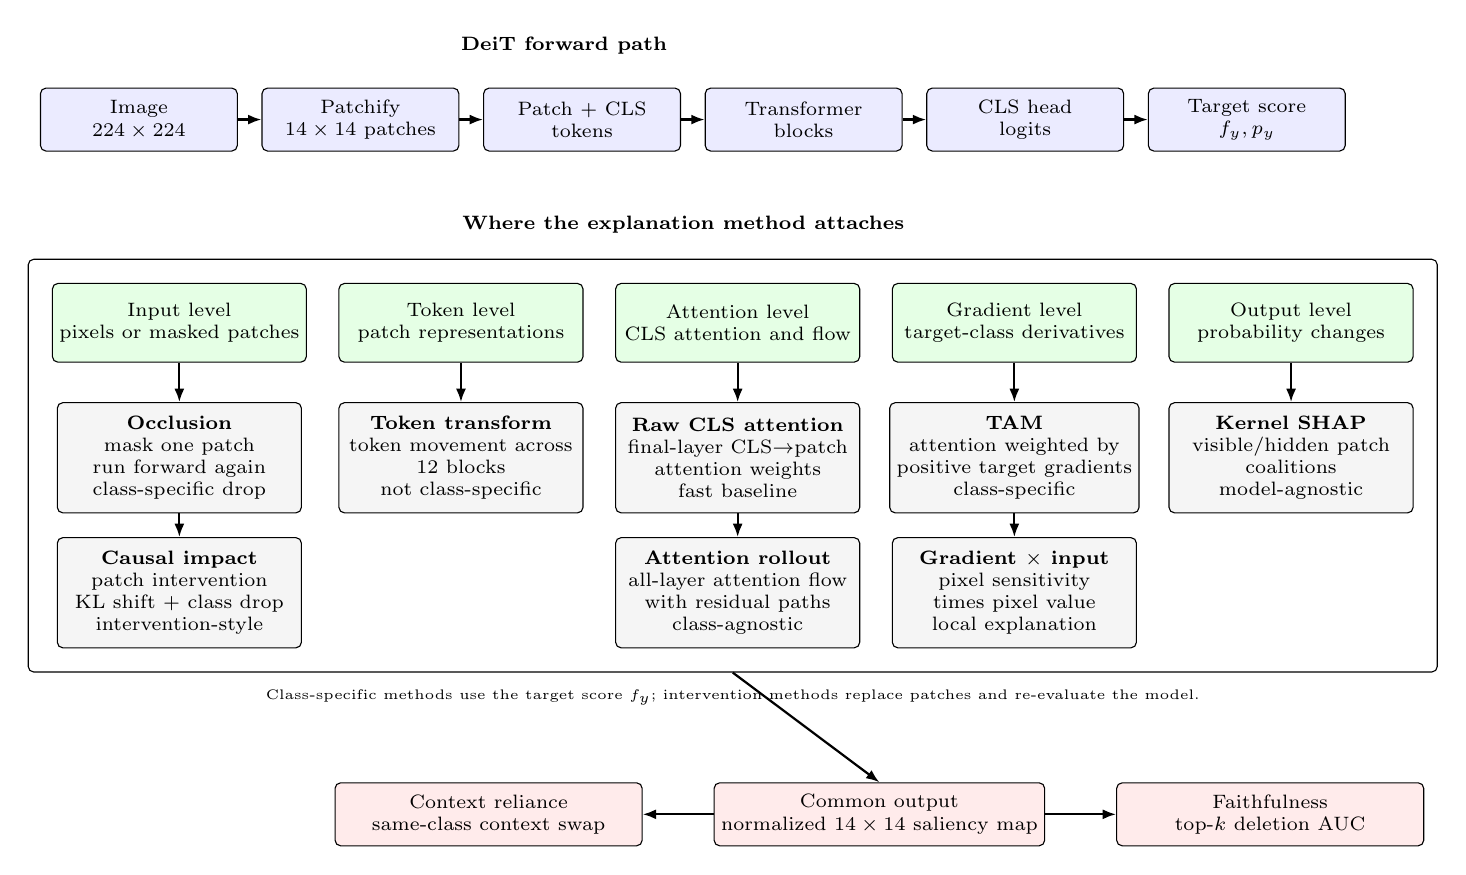
\begin{tikzpicture}[
  font=\scriptsize,
  node distance=4mm and 4mm,
  box/.style={draw, rounded corners=2pt, align=center, minimum height=8mm, inner sep=2.5pt},
  stage/.style={box, fill=blue!8, minimum width=25mm},
  signal/.style={box, fill=green!10, minimum width=31mm, minimum height=10mm},
  method/.style={box, fill=gray!8, minimum width=31mm, minimum height=14mm},
  eval/.style={box, fill=red!8, minimum width=39mm},
  label/.style={align=center, font=\bfseries\scriptsize},
  arr/.style={-{Latex[length=1.7mm]}, thick}]

\node[label] (title) at (0,0) {DeiT forward path};
\node[stage, below=3mm of title, xshift=-54mm] (img) {Image\\$224\times224$};
\node[stage, right=3mm of img] (patch) {Patchify\\$14\times14$ patches};
\node[stage, right=3mm of patch] (tokens) {Patch + CLS\\tokens};
\node[stage, right=3mm of tokens] (blocks) {Transformer\\blocks};
\node[stage, right=3mm of blocks] (logits) {CLS head\\logits};
\node[stage, right=3mm of logits] (score) {Target score\\$f_y,p_y$};
\draw[arr] (img) -- (patch);
\draw[arr] (patch) -- (tokens);
\draw[arr] (tokens) -- (blocks);
\draw[arr] (blocks) -- (logits);
\draw[arr] (logits) -- (score);

\node[label, below=7mm of patch, xshift=41mm] (read) {Where the explanation method attaches};

\node[signal, below=5mm of read, xshift=-64mm] (sinput) {Input level\\pixels or masked patches};
\node[signal, right=4mm of sinput] (stoken) {Token level\\patch representations};
\node[signal, right=4mm of stoken] (sattn) {Attention level\\CLS attention and flow};
\node[signal, right=4mm of sattn] (sgrad) {Gradient level\\target-class derivatives};
\node[signal, right=4mm of sgrad] (sout) {Output level\\probability changes};

\node[method, below=5mm of sinput] (occ) {\textbf{Occlusion}\\mask one patch\\run forward again\\class-specific drop};
\node[method, below=3mm of occ] (cx) {\textbf{Causal impact}\\patch intervention\\KL shift + class drop\\intervention-style};

\node[method, below=5mm of stoken] (tt) {\textbf{Token transform}\\token movement across\\12 blocks\\not class-specific};

\node[method, below=5mm of sattn] (raw) {\textbf{Raw CLS attention}\\final-layer CLS$\to$patch\\attention weights\\fast baseline};
\node[method, below=3mm of raw] (roll) {\textbf{Attention rollout}\\all-layer attention flow\\with residual paths\\class-agnostic};

\node[method, below=5mm of sgrad] (tam) {\textbf{TAM}\\attention weighted by\\positive target gradients\\class-specific};
\node[method, below=3mm of tam] (gxi) {\textbf{Gradient $\times$ input}\\pixel sensitivity\\times pixel value\\local explanation};

\node[method, below=5mm of sout] (shap) {\textbf{Kernel SHAP}\\visible/hidden patch\\coalitions\\model-agnostic};

\draw[arr] (sinput) -- (occ);
\draw[arr] (occ) -- (cx);
\draw[arr] (stoken) -- (tt);
\draw[arr] (sattn) -- (raw);
\draw[arr] (raw) -- (roll);
\draw[arr] (sgrad) -- (tam);
\draw[arr] (tam) -- (gxi);
\draw[arr] (sout) -- (shap);

\node[eval, below=17mm of roll, xshift=18mm] (map) {Common output\\normalized $14\times14$ saliency map};
\node[eval, left=9mm of map] (swap) {Context reliance\\same-class context swap};
\node[eval, right=9mm of map] (del) {Faithfulness\\top-$k$ deletion AUC};

\draw[arr] (map) -- (swap);
\draw[arr] (map) -- (del);

\node[draw, rounded corners=2pt, fit=(sinput)(sout)(cx)(shap), inner sep=3mm] (methodbox) {};
\draw[arr] (methodbox.south) -- (map.north);
\node[font=\tiny, align=center, below=1mm of methodbox] (legend) {Class-specific methods use the target score $f_y$; intervention methods replace patches and re-evaluate the model.};
\end{tikzpicture}
}
\caption{Detailed patch-level XAI map for the DeiT model. Each method is placed at the model signal it uses: input patches, token states, attention matrices, target-class gradients, or output changes. All methods are converted to the same $14\times14$ patch grid before qualitative comparison, deletion-AUC scoring, and context-swap testing.}
\label{fig:xai-method-overview}
\end{figure}

\subsection{Token Transformation}
Token transformation measures how much each patch token changes as it passes through the transformer. For token $i$ in block $\ell$,
\[
\tau_i^{(\ell)}=\|\mathbf{T}^{(\ell)}_i-\mathbf{T}^{(\ell-1)}_i\|_2,\qquad
s_i^{TT}=\sum_{\ell=1}^{12}\tau_i^{(\ell)}.
\]
Here $\mathbf{T}^{(\ell)}_i$ is the embedding of patch token $i$ after transformer block $\ell$. The method therefore compares each token with its previous-layer representation and accumulates the amount of rewriting across all 12 blocks. A patch receives a high score when the transformer repeatedly changes its representation, which usually means that the patch participates strongly in the internal computation.

Token transformation is not class-specific: it does not use the target logit, predicted class, or gradients. It asks where the network worked hardest, not which patches caused class $y$. For NICO++, that matters because high token-transformation scores can come from object shape, background texture, shadows, water, or other scene structure the method cannot distinguish between them. In this report it functions as a representation-flow diagnostic rather than a causal attribution tool.

\subsection{Raw CLS Attention}
Raw CLS attention uses the final transformer block's attention weights from the CLS token to the 196 patch tokens. In DeiT, the CLS token is the summary token passed to the classification head, so its final attention pattern gives a simple view of which image patches are being read by the classifier immediately before prediction. The map is obtained by averaging the final block's attention heads and then reshaping the CLS-to-patch vector to the $14\times14$ patch grid.

Raw attention requires only one forward pass and no gradients, making it fast and visually stable. But it is the weakest attention-based explanation here. It ignores how information flows across layers, how residuals mix representations, and whether a given attention edge actually raises the target logit a patch can receive attention because it is useful for general scene representation, not because it supports the predicted class. In practice, raw attention works as a sanity check: if the final CLS token does not attend anywhere near the object, the model has a problem. If it does, stronger methods are still needed before making a causal claim.

\subsection{Attention Rollout}
Attention rollout composes attention across layers with residual identity mixing \cite{abnar2020quantifying}:
\[
\tilde{\mathbf{A}}^{(\ell)}={1\over2}\left({1\over H}\sum_h\mathbf{A}^{(\ell)}_h+\mathbf{I}\right),
\quad
\mathbf{R}=\tilde{\mathbf{A}}^{(12)}\cdots\tilde{\mathbf{A}}^{(1)}.
\]
The identity matrix $\mathbf{I}$ represents the residual path, and the averaged attention matrix represents token mixing inside each self-attention layer. Multiplying these matrices estimates how information can flow from input patches to the final CLS token through the entire transformer stack. The saliency map is the CLS row of $\mathbf{R}$ after excluding the CLS-to-CLS entry and reshaping the remaining 196 values.

Rollout is stronger than raw final-layer attention because it does not assume the last layer is the only one that matters. A patch that routes information to the CLS token through early or middle blocks can still receive credit. In practice, rollout produces smoother and more object-aligned maps because the multi-layer composition suppresses noise from any single head.

Rollout is still not class-specific. It follows attention flow without asking whether that flow helps or hurts $f_y$, so it can preserve paths that carry context or competing-class evidence. This is why rollout is the best lightweight attention baseline but not the primary method: efficient and often meaningful, but it requires comparison with class-specific scores to be trustworthy.

\subsection{Transition Attention Maps}
TAM adds class specificity by weighting attention with positive gradients \cite{yuan2021tam}:
\[
\bar{\mathbf{A}}^{(\ell)}={1\over H}\sum_h
\mathrm{ReLU}\left({\partial f_y\over\partial \mathbf{A}^{(\ell)}_h}
\odot \mathbf{A}^{(\ell)}_h\right).
\]
The gradient term measures how sensitive the target-class logit is to each attention edge. Multiplying by the attention weight keeps the explanation tied to actual information routing, while the ReLU keeps only positive contributions. In other words, TAM does not simply ask where attention flows; it asks which attention paths positively support class $y$.

After computing these gradient-weighted attention matrices, TAM composes them in rollout fashion to propagate class-relevant influence across layers. The combination is transformer-aware and class-specific: it keeps the multi-layer accounting of rollout while filtering out attention edges that do not support the target. On NICO++ images where object and context evidence coexist, a rollout map may highlight both; TAM narrows the focus to the part of that information flow that raises the target-class logit.

TAM is not a perfect causal intervention local gradients can saturate or become noisy, and the result is a correlation measure rather than a strict causal claim. That said, it is the best-supported method in this study: lowest deletion AUC in Table~\ref{tab:faithfulness} and the most visually focused maps. When TAM highlights object patches and removing those patches sharply lowers confidence, the explanation has both visual and quantitative backing.

\subsection{Occlusion Sensitivity}
Occlusion replaces one patch at a time with the dataset mean baseline and measures the logit or probability drop:
\[
s_i^{occ}=f_y(\mathbf{x})-f_y(\mathbf{x}^{(i)}).
\]
Here $\mathbf{x}^{(i)}$ is the same image after patch $i$ has been replaced. If removing a patch lowers the target logit, the patch is treated as positive evidence for class $y$. If removing it raises the logit, the patch may contain distractor evidence or evidence for another class. In the visualization, positive drops are normalized to form a patch-importance heatmap.

Occlusion is easy to interpret because it is intervention-based. It directly asks what happens when one visible region is removed from the input. This makes it a useful sanity check for attention and gradient methods: if an attention method says a patch is important but occluding that patch has no effect, the attention map is less convincing. Occlusion also has a clear connection to the deletion-AUC protocol used later in the report.

The drawbacks are both practical and conceptual. At $14\times14$, each image needs 196 forward passes slow compared to gradient methods. The mean-color baseline can also be out-of-distribution and create visible patch boundaries. More fundamentally, occlusion tests patches one at a time, missing interactions that ViT decisions may depend on. Still, the interpretation is direct enough to make it worth keeping: a patch matters if removing it changes the prediction.

\subsection{Causal Patch Impact}
Causal patch impact follows the ViT-CX idea of measuring the effect of intervening on a patch \cite{xie2023vitcx}. In this implementation the latent hook falls back to input-space patch replacement, so the score is
\[
s_i^{CX}=\mathrm{KL}(p(\mathbf{x})\|p(\mathbf{x}^{(i)}))+
p_y(\mathbf{x})-p_y(\mathbf{x}^{(i)}).
\]
This score has two terms. The second term is the target-class probability drop, which is similar in spirit to occlusion. The first term is the KL divergence between the full predictive distribution before and after the patch intervention. That term gives credit to patches that change the model's overall belief state, even when the target-class probability drop alone is modest.

Conceptually, causal patch impact is meant to be closer to an intervention than a correlation-based saliency method. A patch is important if changing it changes the model's output distribution. In a full latent-intervention implementation, one could intervene directly on internal patch tokens and separate input artifacts from representation-level causal effects. In this report, the implementation uses input-space patch replacement when latent intervention hooks are unavailable. That makes the method operationally close to occlusion, which explains why the deletion AUC is nearly identical for the two methods.

The method is included because the KL term adds a diagnostic the class-drop alone misses: some patches redistribute probability among competing classes without strongly reducing the true-class score, and those patches matter for understanding failure modes. The interpretation here is appropriately limited causal patch impact is an intervention-style sensitivity score, not a full latent causal explanation.

\subsection{Gradient $\times$ Input}
Gradient $\times$ input scores first-order sensitivity at the input:
\[
s_i^{G\times I}=
\sum_{c,h,w\in \mathrm{patch}_i}x_{c,h,w}
{\partial f_y(\mathbf{x})\over\partial x_{c,h,w}}.
\]
The gradient term measures how a small change in each input pixel would change the target logit. Multiplying by the input value weights this sensitivity by the actual signal present in the image. Pixel-level scores are summed over each $16\times16$ patch to match the ViT patch grid.

The method is fast one forward and backward pass and class-specific: the map is directly tied to $f_y$. It can reveal fine-grained sensitivity that attention methods smooth over. When gradient $\times$ input agrees with TAM on the same patches, both attention flow and local input sensitivity point at the same evidence, which strengthens confidence in both.

The limitation is brittleness: gradients are local derivatives around the exact input, so small perturbations can produce different maps. Multiplying by $x$ also suppresses attribution in dark or low-contrast regions, even when the model is sensitive to those pixels a genuine problem for the \emph{dim} context in NICO++. Gradient $\times$ input is most useful as a local sensitivity diagnostic rather than a causal account.

\subsection{Kernel SHAP}
Kernel SHAP treats each patch as a feature and estimates Shapley values from coalitions \cite{lundberg2017unified}. For coalition $z\in\{0,1\}^{196}$, visible patches are kept and hidden patches are replaced by the mean baseline. The model is evaluated on many such masked images, and a weighted linear surrogate is fit so that each patch receives an estimated contribution to the target prediction.

The appeal of SHAP is its game-theoretic interpretation. In principle, a Shapley value measures a feature's average marginal contribution across all possible feature subsets. This is a stronger conceptual claim than raw attention or gradients because it considers feature interactions through many coalitions. At the patch level, SHAP can identify image regions that consistently help the target class across different masked contexts.

The difficulty is scale: a DeiT image has 196 patch features, making exact Shapley computation infeasible. This report uses 512 sampled coalitions, which is small relative to that feature space. Spatial dependence compounds the problem masking one patch changes the meaning of adjacent patches, and mean replacement produces unnatural images. The noisy maps and weak deletion AUC here are a consequence of budget constraints, not a theoretical failure of Shapley values. More coalitions would likely help, at substantially higher runtime cost.

\subsection{Patch-Level Context Swap and Counterfactuals}
Patch-level context swap is used to test whether highlighted patches carry object evidence or context evidence. For each image, a same-class image from a different context supplies replacement patches. The top 25\% attributed patches are selected from the source image and replaced with corresponding patches from the partner image. The experiment then records the true-class probability drop and whether the predicted class flips.

The protocol holds object identity fixed while changing context. When high-attribution patches transfer cleanly between same-class images, they carry object evidence. When the swap drops confidence or flips the prediction, those patches encode something context-specific either background shortcuts or object-context interactions that do not generalize across scenes. For NICO++, where the same class appears in multiple environments, this distinction is relevant to assessing how much the model relies on scene structure.

Counterfactual perturbation asks a related question: how much must the image change to push the model toward the second-best class? The procedure optimizes a small perturbation under an attribution-derived mask rather than generating a realistic edited image, so it should be read as a model-facing diagnostic. Context swaps and counterfactuals both test whether the regions found by XAI methods actually affect the decision, rather than just correlating with it.

\section{Experimental Results}
\subsection{Classification Performance}
The fine-tuned DeiT reaches 0.9047 top-1 accuracy, 0.9064 macro-F1, and 0.9051 balanced accuracy on the NICO++ test split. The worst context is \emph{dim} at 0.8892, while \emph{grass} is highest at 0.9274 a 3.82-point spread that is easy to miss from aggregate accuracy but large enough to matter for deployment.

For each context $c$, context accuracy is computed over only the test images from that context:
\[
\mathrm{Acc}(c)={\#\{\mathrm{correct\ predictions\ in\ }c\}\over \#\{\mathrm{test\ images\ in\ }c\}}.
\]
Worst-context accuracy is $\min_c \mathrm{Acc}(c)$. It is a conservative robustness metric that aggregate accuracy can mask overall 90.47\% does not reveal that \emph{dim} lags at 88.92\%.

\begin{table}[H]
\centering
\caption{Test performance by context.}
\label{tab:context}
\begin{tabular}{lc}
\toprule
Context & Accuracy\\
\midrule
grass & 0.9274\\
rock & 0.9198\\
autumn & 0.9026\\
water & 0.9016\\
outdoor & 0.8948\\
dim & 0.8892\\
\midrule
overall top-1 & 0.9047\\
macro-F1 & 0.9064\\
\bottomrule
\end{tabular}
\end{table}

\begin{figure}[H]
\centering
\begin{subfigure}[t]{.48\linewidth}
\includegraphics[width=\linewidth]{accuracy.png}\caption{Accuracy}\end{subfigure}
\begin{subfigure}[t]{.48\linewidth}
\includegraphics[width=\linewidth]{macro_f1.png}\caption{Macro-F1}\end{subfigure}\\
\begin{subfigure}[t]{.48\linewidth}
\includegraphics[width=\linewidth]{worst_context_accuracy.png}\caption{Worst context}\end{subfigure}
\begin{subfigure}[t]{.48\linewidth}
\includegraphics[width=\linewidth]{token_transformation_by_layer.png}\caption{Token rewriting}\end{subfigure}
\caption{Training and representation summaries. The model converges smoothly, while token transformation peaks in early and late-middle blocks.}
\label{fig:training-repr}
\end{figure}

\subsection{Faithfulness}
Deletion AUC removes the top-ranked patches for $k\in\{5,10,20,30,50\}\%$ and integrates the remaining target probability. Lower AUC means the method found patches whose removal most damages the prediction.

\begin{table}[H]
\centering
\caption{Faithfulness by top-$k$ deletion AUC on 200 stratified samples. Lower is better.}
\label{tab:faithfulness}
\begin{tabular}{lcc}
\toprule
Method & AUC & Std.\\
\midrule
TAM & \textbf{0.1579} & 0.1711\\
Attention rollout & 0.2022 & 0.1850\\
Token transformation & 0.2236 & 0.1926\\
Causal patch impact & 0.2264 & 0.1941\\
Occlusion & 0.2264 & 0.1941\\
Gradient $\times$ input & 0.2265 & 0.2021\\
Kernel SHAP & 0.2562 & 0.2091\\
\bottomrule
\end{tabular}
\end{table}

TAM leads by a clear margin AUC 21.9\% lower than attention rollout and 38.4\% lower than SHAP. This fits its design: gradient filtering keeps only the attention paths that positively affect the target logit. Attention rollout is the strongest parameter-free method, which suggests the fine-tuned DeiT does route useful evidence through CLS attention in most correct predictions. Occlusion, causal impact, and gradient $\times$ input are nearly tied, confirming that their input-space sensitivity signals overlap on this model. SHAP performs worst: 512 coalitions are too few for stable Shapley estimation over 196 correlated patches.

\begin{figure}[H]
\centering

\includegraphics[width=.98\linewidth]{deletion_curves_top.png}
\caption{Top-$k$ deletion curves. TAM removes the most causally important patches fastest, producing the lowest target-probability curve.}
\label{fig:deletion}
\end{figure}

\subsection{Sample Protocol for Method Results}
Each method is reported independently using the same six representative samples: \emph{cactus/dim}, \emph{airplane/autumn}, \emph{crab/dim}, \emph{horse/water}, \emph{fishing rod/water}, and \emph{train/autumn}. This gives every method its own result figure and analysis while keeping the comparison fair. The six cases include low-light, canonical object-centered, small-object, animal, vehicle, and water-context examples, so the visual comparison is not driven by a single easy sample.

\subsection{Token Transformation Results}
Token transformation shows where the transformer rewrites patch representations most strongly, not where class evidence is causal. In Fig.~\ref{fig:tt-results}, the cactus and airplane samples concentrate token changes on the object silhouette the ViT is spending representational capacity on object structure. The crab and horse samples are broader, with changes extending into surrounding dim or water texture: the model has to process both the object and its background before settling on the final class representation. The fishing-rod case highlights an additional constraint: a thin object occupying few patches forces representation change to spread into nearby scene structure because the transformer needs surrounding context to stabilize a narrow target. The train is more object-aligned a large rigid vehicle gives the model enough patches to work with. This pattern explains the middle-ranked deletion AUC: token transformation captures important processing regions, but those regions include context alongside object.

\inplacesix{sample_00010732_token_transformation_overlay.png}{sample_00000001_token_transformation_overlay.png}{sample_00012227_token_transformation_overlay.png}{sample_00079663_token_transformation_overlay.png}{sample_00076958_token_transformation_overlay.png}{sample_00008127_token_transformation_overlay.png}{Token transformation results. Bright patches are tokens with the largest cumulative representation change across transformer blocks.}{fig:tt-results}

\subsection{Raw CLS Attention Results}
Raw final-layer CLS attention in Fig.~\ref{fig:rawattn-results} is stable and easy to interpret but spreads across too much of the image to be useful on its own. The cactus case attends near the object body but does not cleanly separate the cactus from the dim surround. The airplane is better aligned with the fuselage. The crab, horse, and fishing-rod cases spread attention across both object and surrounding scene. The train is the cleanest case a long rigid body gives the CLS token a strong spatial anchor. In all cases, raw attention shows where the final CLS token looks, not which patches actually raise the target logit.

\inplacesix{sample_00010732_last_layer_cls_attention.png}{sample_00000001_last_layer_cls_attention.png}{sample_00012227_last_layer_cls_attention.png}{sample_00079663_last_layer_cls_attention.png}{sample_00076958_last_layer_cls_attention.png}{sample_00008127_last_layer_cls_attention.png}{Raw CLS attention results from the final transformer block. The maps are stable but not class-discriminative.}{fig:rawattn-results}

\subsection{Attention Rollout Results}
Rollout composes attention through all transformer blocks and usually produces cleaner maps than final-layer attention. In Fig.~\ref{fig:rollout-results}, it tracks the cactus body and airplane fuselage well and stays reasonably localized on the crab and train. The horse and fishing-rod water-context samples are less clean: rollout keeps object evidence but also preserves paths through surrounding water and scene patches. The deletion AUC of 0.2022 is second-best many rollout-ranked patches are genuinely important to the prediction. The persistent weakness is that rollout is class-agnostic: it follows attention flow without asking whether that flow supports the target class, which is why TAM consistently outperforms it.

\inplacesix{sample_00010732_rollout_overlay.png}{sample_00000001_rollout_overlay.png}{sample_00012227_rollout_overlay.png}{sample_00079663_rollout_overlay.png}{sample_00076958_rollout_overlay.png}{sample_00008127_rollout_overlay.png}{Attention rollout results. Composing attention across layers improves localization compared with raw final-layer attention.}{fig:rollout-results}

\subsection{TAM Results}
TAM is the strongest method in both qualitative and quantitative terms. In Fig.~\ref{fig:tam-results}, the maps are the most tightly object-centered: cactus body, airplane fuselage, crab region, and train body all receive concentrated heat. On the water-context horse and fishing-rod samples, TAM still localizes the object more cleanly than rollout, though some high-scoring patches remain in the surrounding scene. This residual context signal is worth noting rather than explaining away even the best method reveals that the classifier mixes object and context evidence when the scene is distinctive. With a deletion AUC of 0.1579, removing TAM's top patches collapses target probability faster than any other method. TAM is the primary explanation method for this model.

\inplacesix{sample_00010732_tam_overlay.png}{sample_00000001_tam_overlay.png}{sample_00012227_tam_overlay.png}{sample_00079663_tam_overlay.png}{sample_00076958_tam_overlay.png}{sample_00008127_tam_overlay.png}{TAM results. Positive gradient-weighted attention produces the most faithful and visually focused patch maps.}{fig:tam-results}

\subsection{Occlusion Results}
Occlusion maps in Fig.~\ref{fig:occ-results} are blockier than attention-based ones each probe operates on a discrete $16\times16$ patch but the interpretation is direct. The airplane result is the most intuitive: fuselage and wing regions matter most. The cactus stays object-aligned, though the dim background introduces some scattered sensitivity. The crab and horse results spread into context; removing dim-scene or water-adjacent patches also lowers confidence. The fishing-rod sample is especially sensitive to nearby background because the thin object has few exclusive patches. Occlusion is a useful sanity check, but at 196 forward passes per image it is slow, and its AUC of 0.2264 falls well behind TAM.

\inplacesix{sample_00010732_occlusion_overlay.png}{sample_00000001_occlusion_overlay.png}{sample_00012227_occlusion_overlay.png}{sample_00079663_occlusion_overlay.png}{sample_00076958_occlusion_overlay.png}{sample_00008127_occlusion_overlay.png}{Occlusion sensitivity results. High-saliency patches are those whose removal most reduces target evidence.}{fig:occ-results}

\subsection{Causal Patch Impact Results}
Causal patch impact is designed to measure the distributional effect of intervening on each patch, but because this run uses an input-space fallback, Fig.~\ref{fig:causal-results} looks nearly identical to occlusion the deletion AUC matches as well at 0.2264. The added KL term provides a slightly broader view: a patch that redistributes probability across classes without strongly reducing the true-class score will still score high. But the visual maps do not differ enough to change any conclusions. True latent-token intervention would be needed to make causal patch impact meaningfully distinct from occlusion.

\inplacesix{sample_00010732_causal_impact_overlay.png}{sample_00000001_causal_impact_overlay.png}{sample_00012227_causal_impact_overlay.png}{sample_00079663_causal_impact_overlay.png}{sample_00076958_causal_impact_overlay.png}{sample_00008127_causal_impact_overlay.png}{Causal patch impact results. With input-space fallback, the maps behave similarly to occlusion but include distribution-shift information.}{fig:causal-results}

\subsection{Gradient $\times$ Input Results}
Gradient $\times$ input is fast and class-specific, but unreliable in several of these samples. The dim cactus gets weaker and more fragmented attribution because the score multiplies gradients by low-magnitude pixels. The airplane and train are sharper stronger contrast and larger coherent shapes help. The crab, horse, and fishing-rod maps scatter across both object and texture. With deletion AUC 0.2265 and lower stability than rollout under Gaussian noise, this method is best used as a secondary diagnostic: when gradient maps agree with TAM, both attention flow and local sensitivity support the same evidence; when they fragment, the sample is locally unstable and deserves closer inspection.

\inplacesix{sample_00010732_patch_heatmap.png}{sample_00000001_patch_heatmap.png}{sample_00012227_patch_heatmap.png}{sample_00079663_patch_heatmap.png}{sample_00076958_patch_heatmap.png}{sample_00008127_patch_heatmap.png}{Gradient $\times$ input results. The method is class-specific but brittle, especially in low-light and context-heavy samples.}{fig:grad-results}

\subsection{Kernel SHAP Results}
Kernel SHAP maps in Fig.~\ref{fig:shap-results} are visibly noisier than TAM or rollout. The airplane and train still show object signal strong visual structure helps the coalition sampling converge but the cactus, crab, horse, and fishing-rod maps scatter high values in ways that are hard to interpret. SHAP has the worst deletion AUC at 0.2562. The six-sample panel makes the reason clear: 512 coalitions are not enough for stable Shapley estimation over 196 correlated patches. SHAP is not theoretically weak, just underpowered here. A larger coalition budget would likely improve the maps, at considerably higher runtime cost.

\inplacesix{sample_00010732_shap_overlay.png}{sample_00000001_shap_overlay.png}{sample_00012227_shap_overlay.png}{sample_00079663_shap_overlay.png}{sample_00076958_shap_overlay.png}{sample_00008127_shap_overlay.png}{Kernel SHAP results. At the tested coalition budget, maps are noisy and least faithful by deletion AUC.}{fig:shap-results}

\subsection{Context Swap and Counterfactual Results}
Across 200 same-class cross-context pairs, the mean probability drop is 0.061 and the median is near zero, but 20\% of swaps flip the predicted class. The largest average drop is in \emph{water} at 0.2299, suggesting that water patches are highly predictive in NICO++ several classes are strongly associated with marine settings, and the model appears to have picked up on it.

\begin{table}[H]
\centering
\caption{True-class probability drop after patch-level context swap.}
\label{tab:swap}
\begin{tabular}{lc}
\toprule
Source context & Mean drop\\
\midrule
water & \textbf{0.2299}\\
outdoor & 0.0883\\
dim & 0.0697\\
rock & 0.0511\\
grass & 0.0467\\
autumn & 0.0254\\
\bottomrule
\end{tabular}
\end{table}

\begin{figure}[H]
\centering
\begin{subfigure}[t]{.48\linewidth}
\includegraphics[width=\linewidth]{context_swap_drop_by_context.png}\caption{Drop by context}\end{subfigure}
\begin{subfigure}[t]{.48\linewidth}
\includegraphics[width=\linewidth]{context_swap_probability_drop_hist.png}\caption{Drop histogram}\end{subfigure}
\caption{Context-swap results over 200 pairs. Water is the strongest context shortcut.}
\label{fig:swap}
\end{figure}

\inplacetriplet{sample_00010732_context_proxy_overlay.png}{sample_00000001_context_proxy_overlay.png}{sample_00012227_context_proxy_overlay.png}{Context-swap masks. The highlighted regions are the top-attributed patches selected for cross-context replacement.}{fig:context-mask-results}

\inplacetriplet{sample_00010732_context_swapped.png}{sample_00000001_context_swapped.png}{sample_00012227_context_swapped.png}{Context-swapped samples. These images test whether the selected patches carry transferable object evidence or context evidence.}{fig:context-swapped-results}

\inplacetriplet{sample_00010732_counterfactual.png}{sample_00000001_counterfactual.png}{sample_00012227_counterfactual.png}{Counterfactual perturbation samples. Perturbations that shift the prediction concentrate near the same evidence-bearing regions found by the stronger attribution methods.}{fig:counterfactual-results}

\subsection{Stability and Representation Behavior}
Stability is measured under Gaussian input noise ($\sigma=0.05$) on 20 samples and three seeds. Attention rollout is highly stable with Spearman $\rho=0.997$ and top-10\% overlap 0.922. Gradient $\times$ input is less stable with $\rho=0.898$ and overlap 0.679, consistent with gradients being local first-order responses to input perturbations.

Representation metrics follow a depth pattern. CLS top-10\% concentration rises from roughly 0.18 in early blocks to 0.57 in the final block the classifier increasingly narrows its evidence base as depth increases. Head diversity peaks in middle layers, where different heads specialize, and then collapses near the output as the CLS token aggregates class evidence. This depth pattern is consistent with the qualitative panels: correct predictions tend to lock onto object patches before the final blocks, while shortcut predictions lock onto context patches and amplify them.

\begin{figure}[H]
\centering
\begin{subfigure}[t]{.48\linewidth}
\includegraphics[width=\linewidth]{stability_summary.png}\caption{Stability}\end{subfigure}
\begin{subfigure}[t]{.48\linewidth}
\includegraphics[width=\linewidth]{cls_concentration_by_layer.png}\caption{CLS concentration}\end{subfigure}\\
\begin{subfigure}[t]{.48\linewidth}
\includegraphics[width=\linewidth]{entropy_by_layer.png}\caption{Entropy}\end{subfigure}
\begin{subfigure}[t]{.48\linewidth}
\includegraphics[width=\linewidth]{head_diversity_by_layer.png}\caption{Head diversity}\end{subfigure}
\caption{Explanation stability and internal ViT behavior. Attention rollout is stable under noise; CLS evidence becomes more concentrated with depth.}
\label{fig:axes}
\end{figure}

\section{Discussion}
\textbf{Overall finding.} The DeiT model is accurate but not context-invariant. The 90.47\% top-1 accuracy and 0.9064 macro-F1 show that the model has learned strong object representations, but the per-context spread, deletion curves, and context-swap results all show that background evidence still influences decisions and aggregate accuracy does not reveal this.

\textbf{TAM is the strongest default.} TAM wins on both metrics. It extends rollout by filtering attention through target-class gradients, which matters on NICO++ where object and context evidence coexist in the same image. The deletion-AUC ranking confirms the maps are more than visually plausible: TAM's top patches are the most damaging to remove, putting its explanations closer to causal than the alternatives.

\textbf{Raw attention is not enough.} Raw CLS attention is stable and visually useful, but it ignores residual flow and target-class gradients. It can show where the final CLS token looks, not necessarily which patches caused the target class.

\textbf{Perturbation methods are good sanity checks.} Occlusion and causal patch impact have direct causal interpretations, but they are slow and can create unnatural masked images. Their near-identical AUC values show that the current causal-impact implementation behaves like occlusion because it falls back to input-space ablation.

\textbf{SHAP needs a larger budget.} SHAP is theoretically attractive, but the tested 512-coalition setting is underpowered for 196 dependent patch features. Its maps are noisy and its AUC is worst. A much larger coalition budget may improve quality, but with substantial runtime cost.

\textbf{Context dependence remains after high accuracy.} Many predictions are genuinely object-centered the model has not simply memorized backgrounds. But the water swap result and the water-context horse and fishing-rod samples show that context still influences decisions. The same-object panels make this concrete: cactus, horse, fishing rod, and train explanations shift when the background changes, especially in water-like settings. Aggregate accuracy hides this localized reliance.

\textbf{Practical implication.} For a deployment audit, picking a single saliency map and stopping is not enough. A more complete workflow: evaluate per context first; generate TAM as the primary explanation; compare against rollout and perturbation methods; run deletion AUC to validate faithfulness; and check same-object cross-context panels to see whether evidence drifts from object to background. Visual inspection alone misses too much.

\section{Limitations}
NICO++ does not provide pixel-level object masks, so object-versus-background attribution is assessed qualitatively and through context swaps rather than exact segmentation metrics. The causal patch impact method falls back to input-space ablation, which makes it redundant with occlusion in this run. SHAP uses 512 coalitions due to runtime constraints; a larger budget could change its ranking. Counterfactual perturbations are model-facing diagnostics and should not be read as human-realistic edited images. The analysis covers one DeiT-Small/16 checkpoint; results for larger ViTs or context-balanced training may differ.

\clearpage
\section{Same Object Across Different Contexts}
\label{sec:same-object}
This section compares the same object class across multiple contexts the most direct visual test in the report. The class label is fixed while the surrounding scene changes. A perfectly object-centered model would show the same explanation across all contexts; when the explanation shifts, the classifier is using background or scene evidence as part of its decision.

These panels ask a different question than the earlier method-comparison figures. Rather than asking which XAI method is most faithful, the question here is whether the same method explains the same object consistently when the background changes. TAM is the primary method because it had the best deletion AUC and the cleanest localization; attention rollout is included for cactus as a reference baseline to show how much broader the explanation becomes without target-gradient filtering. The key diagnostic is not whether any object signal appears nearly all correct predictions contain some but whether the highest-evidence patches stay on the object or drift into context-specific regions.

\subsection{Cactus Across Six Contexts}
Fig.~\ref{fig:cactus-tam-contexts} compares \emph{cactus} across all six NICO++ contexts: \emph{autumn}, \emph{dim}, \emph{grass}, \emph{rock}, \emph{water}, and \emph{outdoor}. TAM stays mostly on the cactus body in the dim, grass, rock, and outdoor cases object shape rather than background is driving the prediction. The dim example is notable: even under low contrast, the highlighted region follows the cactus silhouette rather than spreading across the dark scene.

The water-context case is less clean. The heatmap still reaches the cactus, but surrounding scene patches receive more emphasis than in the other five contexts consistent with water producing the largest true-class probability drop in the swap experiment. Cactus predictions are usually object-driven, but water redistributes the evidence enough that background patches become meaningfully involved.

\begin{center}
\begin{minipage}[t]{.16\linewidth}\centering
\includegraphics[width=\linewidth]{sample_00000951_tam_overlay.png}\\[-1pt]\footnotesize (a) Autumn\end{minipage}\hfill
\begin{minipage}[t]{.16\linewidth}\centering
\includegraphics[width=\linewidth]{sample_00010732_tam_overlay.png}\\[-1pt]\footnotesize (b) Dim\end{minipage}\hfill
\begin{minipage}[t]{.16\linewidth}\centering
\includegraphics[width=\linewidth]{sample_00024386_tam_overlay.png}\\[-1pt]\footnotesize (c) Grass\end{minipage}\hfill
\begin{minipage}[t]{.16\linewidth}\centering
\includegraphics[width=\linewidth]{sample_00060245_tam_overlay.png}\\[-1pt]\footnotesize (d) Rock\end{minipage}\hfill
\begin{minipage}[t]{.16\linewidth}\centering
\includegraphics[width=\linewidth]{sample_00071905_tam_overlay.png}\\[-1pt]\footnotesize (e) Water\end{minipage}\hfill
\begin{minipage}[t]{.16\linewidth}\centering
\includegraphics[width=\linewidth]{sample_00043620_tam_overlay.png}\\[-1pt]\footnotesize (f) Outdoor\end{minipage}
\captionof{figure}{Same object, different contexts using TAM: cactus in six settings. TAM is object-focused in most contexts but shows more context leakage in water.}
\label{fig:cactus-tam-contexts}
\end{center}

Attention rollout in Fig.~\ref{fig:cactus-rollout-contexts} shows the same trend but less sharply. Without gradient weighting, rollout preserves broader information flow through the CLS token all six images route information from the cactus region, but water and outdoor backgrounds look more influential than they do in the TAM maps. The side-by-side comparison makes the case for gradient weighting: rollout answers the question of where information flows; TAM answers the narrower question of which patches support the target class.

\begin{center}
\begin{minipage}[t]{.16\linewidth}\centering
\includegraphics[width=\linewidth]{sample_00000951_rollout_overlay.png}\\[-1pt]\footnotesize (a) Autumn\end{minipage}\hfill
\begin{minipage}[t]{.16\linewidth}\centering
\includegraphics[width=\linewidth]{sample_00010732_rollout_overlay.png}\\[-1pt]\footnotesize (b) Dim\end{minipage}\hfill
\begin{minipage}[t]{.16\linewidth}\centering
\includegraphics[width=\linewidth]{sample_00024386_rollout_overlay.png}\\[-1pt]\footnotesize (c) Grass\end{minipage}\hfill
\begin{minipage}[t]{.16\linewidth}\centering
\includegraphics[width=\linewidth]{sample_00060245_rollout_overlay.png}\\[-1pt]\footnotesize (d) Rock\end{minipage}\hfill
\begin{minipage}[t]{.16\linewidth}\centering
\includegraphics[width=\linewidth]{sample_00071905_rollout_overlay.png}\\[-1pt]\footnotesize (e) Water\end{minipage}\hfill
\begin{minipage}[t]{.16\linewidth}\centering
\includegraphics[width=\linewidth]{sample_00043620_rollout_overlay.png}\\[-1pt]\footnotesize (f) Outdoor\end{minipage}
\captionof{figure}{Same object, different contexts using attention rollout. Rollout remains useful, but it is broader than TAM and includes more background evidence.}
\label{fig:cactus-rollout-contexts}
\end{center}

\subsection{Horse Across Four Contexts}
Fig.~\ref{fig:horse-tam-contexts} shows \emph{horse} across autumn, outdoor, rock, and water. Unlike the cactus, a horse is deformable and varies in pose, so the model cannot rely on a fixed silhouette. TAM highlights the animal body in the autumn and outdoor examples, which suggests the model has learned real object structure rather than memorizing scene type. The rock example is mostly object-centered, though some attribution spreads into high-texture background regions where rock surface competes visually with the animal boundary.

Water context again produces a less clean explanation: the map does not collapse into background entirely, but it loses some of its object focus. Water is not a defining feature of the class \emph{horse}, so any reliance on water-like patches is a shortcut. The pattern is the same as with cactus context leakage is not a property of any particular object.

\begin{center}
\begin{minipage}[t]{.24\linewidth}\centering
\includegraphics[width=\linewidth]{sample_00004344_tam_overlay.png}\\[-1pt]\footnotesize (a) Autumn\end{minipage}\hfill
\begin{minipage}[t]{.24\linewidth}\centering
\includegraphics[width=\linewidth]{sample_00050099_tam_overlay.png}\\[-1pt]\footnotesize (b) Outdoor\end{minipage}\hfill
\begin{minipage}[t]{.24\linewidth}\centering
\includegraphics[width=\linewidth]{sample_00063825_tam_overlay.png}\\[-1pt]\footnotesize (c) Rock\end{minipage}\hfill
\begin{minipage}[t]{.24\linewidth}\centering
\includegraphics[width=\linewidth]{sample_00079663_tam_overlay.png}\\[-1pt]\footnotesize (d) Water\end{minipage}
\captionof{figure}{Same object, different contexts using TAM: horse in autumn, outdoor, rock, and water settings.}
\label{fig:horse-tam-contexts}
\end{center}

\subsection{Fishing Rod Across Three Contexts}
Fig.~\ref{fig:fishing-rod-tam-contexts} shows \emph{fishing rod} across autumn, grass, and water. The fishing rod occupies less image area than the surrounding scene, so the model has fewer dedicated object patches to anchor on. TAM highlights the rod and nearby handle region in the autumn and grass cases, though the narrow shape leaves more room for context to enter the map.

The water case activates more surrounding context than the autumn and grass cases, consistent with what was seen for cactus and horse. The issue is partly geometric: when an object occupies a small fraction of the image, even a faithful method may reveal that nearby scene structure is helping the classifier stabilize the prediction.

\begin{center}
\begin{minipage}[t]{.31\linewidth}\centering
\includegraphics[width=\linewidth]{sample_00002828_tam_overlay.png}\\[-1pt]\footnotesize (a) Autumn\end{minipage}\hfill
\begin{minipage}[t]{.31\linewidth}\centering
\includegraphics[width=\linewidth]{sample_00028586_tam_overlay.png}\\[-1pt]\footnotesize (b) Grass\end{minipage}\hfill
\begin{minipage}[t]{.31\linewidth}\centering
\includegraphics[width=\linewidth]{sample_00076958_tam_overlay.png}\\[-1pt]\footnotesize (c) Water\end{minipage}
\captionof{figure}{Same object, different contexts using TAM: fishing rod in autumn, grass, and water settings.}
\label{fig:fishing-rod-tam-contexts}
\end{center}

\subsection{Train Across Four Contexts}
Fig.~\ref{fig:train-tam-contexts} shows \emph{train} across autumn, grass, rock, and water. Trains are large and rigid, which makes object-centered attribution easier. In the grass and rock cases, TAM stays mainly on the train body, following the long rectangular shape and high-contrast vehicle parts even as the surrounding terrain changes.

The water case shows broader saliency around scene structure. The train is still visible in the explanation, but context has become part of the evidence. Context reliance appears to be class-dependent: large structured objects like trains are easier to explain in object-centered terms, but even they show some attribution drift in distinctive contexts.

\begin{center}
\begin{minipage}[t]{.24\linewidth}\centering
\includegraphics[width=\linewidth]{sample_00008127_tam_overlay.png}\\[-1pt]\footnotesize (a) Autumn\end{minipage}\hfill
\begin{minipage}[t]{.24\linewidth}\centering
\includegraphics[width=\linewidth]{sample_00040520_tam_overlay.png}\\[-1pt]\footnotesize (b) Grass\end{minipage}\hfill
\begin{minipage}[t]{.24\linewidth}\centering
\includegraphics[width=\linewidth]{sample_00068812_tam_overlay.png}\\[-1pt]\footnotesize (c) Rock\end{minipage}\hfill
\begin{minipage}[t]{.24\linewidth}\centering
\includegraphics[width=\linewidth]{sample_00087551_tam_overlay.png}\\[-1pt]\footnotesize (d) Water\end{minipage}
\captionof{figure}{Same object, different contexts using TAM: train in autumn, grass, rock, and water settings.}
\label{fig:train-tam-contexts}
\end{center}

\subsection{Cross-Object Interpretation}
Across cactus, horse, fishing rod, and train, the same pattern holds with varying intensity. TAM usually stays on the object, which is why the classifier is accurate overall. But the maps are not background-invariant: water and outdoor scenes pull saliency away from the object more than other contexts, and high-texture surfaces can also pull attribution toward background. Four object categories showing the same trend makes the case more convincingly than any single example.

Context dependence is not a binary property. Every object panel shows some object-centered evidence, so the model is not simply a background classifier. But the same object receives different explanations across contexts, so it is not purely object-centered either. The mixture of object and context evidence shifts with class, object size, shape, and scene type. That is why cross-context XAI panels matter: a single correct prediction with a clean heatmap is not enough evidence of robust object reasoning.

\section{Conclusion}
A high-performing DeiT-Small/16 on NICO++ still uses context as evidence in measurable ways. The model reaches 90.47\% accuracy and 0.9064 macro-F1, but worst-context accuracy drops to 88.92\% and 20\% of patch-level context swaps flip predictions. TAM is the best explanation method by deletion AUC and by visual inspection: it produces the most faithful and focused maps. Attention rollout is the strongest lightweight alternative; occlusion and causal patch impact work as sanity checks; gradient $\times$ input is fast but brittle; and SHAP needs a larger coalition budget to be useful.

The same-object comparisons make the finding concrete: when the object label stays fixed and only the context changes, explanations shift. Cactus, horse, fishing rod, and train all show stronger background leakage in at least one context, with water-like scenes as the most consistent source consistent with the swap experiment's finding that water is the strongest shortcut context. Aggregate accuracy is not enough for a deployment audit. The more informative workflow is to evaluate per context, use TAM as the primary explanation, validate it against rollout and perturbation methods, and check same-object cross-context panels before concluding that the model reasons about objects rather than scenes.

\begin{thebibliography}{99}\small

\bibitem{dosovitskiy2021image}
A.~Dosovitskiy et al., ``An Image is Worth 16x16 Words: Transformers for Image Recognition at Scale,'' \emph{ICLR}, 2021.

\bibitem{touvron2021training}
H.~Touvron et al., ``Training data-efficient image transformers and distillation through attention,'' \emph{ICML}, 2021.

\bibitem{abnar2020quantifying}
S.~Abnar and W.~Zuidema, ``Quantifying Attention Flow in Transformers,'' \emph{ACL}, 2020.

\bibitem{chefer2021transformer}
H.~Chefer, S.~Gur, and L.~Wolf, ``Transformer Interpretability Beyond Attention Visualization,'' \emph{CVPR}, 2021.

\bibitem{zhang2023nico}
X.~Zhang et al., ``NICO++: Towards Better Benchmarking for Domain Generalization,'' \emph{CVPR}, 2023.

\bibitem{lundberg2017unified}
S.~M.~Lundberg and S.-I.~Lee, ``A Unified Approach to Interpreting Model Predictions,'' \emph{NeurIPS}, 2017.

\bibitem{selvaraju2017gradcam}
R.~R.~Selvaraju et al., ``Grad-CAM: Visual Explanations from Deep Networks via Gradient-based Localization,'' \emph{ICCV}, 2017.

\bibitem{yuan2021tam}
T.~Yuan et al., ``Explaining Information Flow Inside Vision Transformers Using Transition Attention Maps,'' \emph{NeurIPS}, 2021.

\bibitem{xie2023vitcx}
W.~Xie, X.-H.~Li, C.~C.~Cao, and N.~L.~Zhang, ``ViT-CX: Causal Explanation of Vision Transformers,'' \emph{IJCAI}, 2023.

\bibitem{geirhos2020shortcut}
R.~Geirhos et al., ``Shortcut Learning in Deep Neural Networks,'' \emph{Nature Machine Intelligence}, 2020.

\end{thebibliography}

\end{document}
